\section{Composing Monads}
\label{composing_monads}

Questo è il capitolo principale dell'intero report, espone il concetto più
interessante della composizione dei \textit{Monads}, prima di procedere
definiamo in maniera naturale la composizione per \textit{Functor} e
\textit{Premonads}.
Poi proviamo a trovare la composizione naturale anche per i \textit{Monads} e
daremo una dimostrazione formale di non esistenza
\ref{natural_join_doesn_t_exist}.
Quindi cercheremo di classificare quali condizioni sono necessarie per
comporre due \textit{Monads} $M$ e $N$.

\subsection{Conditions for Composition}
\label{conditions_for_composition}

Supponiamo che $M$ e $N$ siano $Functors$, per eliminare a priori la confusione
generata da quale $map$ applico di volta in volta, scriverò $map_M$ e $map_N$
per ogni caso.
Ora possiamo pensare alla composizione di $M$ e $N$ com un tipo costruttore che
riceve $a$ come parametro (senza restrizioni di tipo, $a$ può avere qualiasi
tipo) e costruisce il tipo $M\ (N\ a)$.
Per questo nuovo tipo l'operatore $map$ avrà la seguente firma.
\begin{align*}
  map\ ::\ (a \to b) \to (M\ (N\ a) \to M\ (N\ b))
\end{align*}
Fortunatamente è molto semplice trovare una funzione che soddisfi la firma
utilizzando il fatto che $M$ e $N$ siano funtori
\begin{align*}
  map\ =\ map_M\ .\ map_N
\end{align*}
Questa funzione soddisfa le leggi $(M1)$ e $(M2)$
\begin{framed}
  \begin{align*}
      (M1)\qquad
      &\quad map\ id && \{map\}\\
      =&\quad map_M\ (map_N\ id) && \{M1_N\}\\
      =&\quad map_M id && \{M1_M\}\\
      =&\quad id && \\\\
      (M2)\qquad
      &\quad map\ f\ .\ map\ g && \{map, map\}\\
      =&\quad map_M\ (map_N\ f)\ .\ map_M\ (map_N\ g) && \{M2_M\}\\
      =&\quad map_M\ (map_N\ f\ .\ map_N\ g) && \{M2_N\}\\
      =&\quad map_M\ (map_N\ (f\ .\ g)) && \{map\}\\
      =&\quad map\ (f\ .\ g)
    %\caption*{$(M1)$}
  \end{align*}
\end{framed}
La composizione di due $Premonads$ arbitrari è simile, dobbiamo trovare una
funzione che abbia la firma
\begin{align*}
  unit\ ::\ a \to M\ (N\ a)
\end{align*}
Come per il precedente caso viene banalmente
\begin{align*}
  unit\ =\ unit_M\ .\ unit_N
\end{align*}
Questa funzione soddisfa la legge $(M3)$
\begin{framed}
  \begin{align*}
      (M3)\qquad
      &\quad unit\ .\ f && \{unit\}\\
      =&\quad unit_M\ .\ unit_N\ .\ f && \{M3_N\}\\
      =&\quad unit_M\ .\ map_N\ f\ .\ unit_N && \{M3_M\}\\
      =&\quad map_M\ (map_N\ f)\ .\ unit_M .\ unit_N && \{map, unit\}\\
      =&\quad map\ f\ .\ unit
  \end{align*}
\end{framed}
Sfortunatamente lo stesso meccanismo non può essere ripetuto per comporre due
$Monads$ difatti dovremmo trovare una funzione dalla seguente firma
\begin{align*}
  join\ ::\ M\ (N\ (M\ (N\ a))) \to M\ (N\ a)
\end{align*}
Che soddisfi le leggi $(M4\dots7)$.
Come prima prova potremmo definire il $join$ come composizione naturale
ottenendo $join\ =\ join_M\ .\ join_N$, questa funzione però non è tipata
correttamente se $M$ e $N$ sono diversi tra loro.
Infatti non c'è nessun modo di costruire la funzione $join$ con il tipo sopra
descritto usando solamente le operazioni dei due $Monads$.
La dimostrazione formale è data in appendice \ref{natural_join_doesn_t_exist}.\newline

Procedo quindi aggiungendo requisiti per poter ampliare le condizioni per la
composizione, difatti è possibile generalizzare la composizione tra $Monads$
richiedendo insieme ai $Monads$ o $Premonads$ $M$ e $N$ anche una funzione
ausiliaria per l'implementazione di $join$.

\subsection{Prod Construction}
\label{prod_construction}

La composizione di un monade $M$ con un premonade $N$ è un monade se è definita
una funzione
\begin{equation*}
  prod\ ::\ N\ (M  (N  a)) \to M\ (N\ a)
\end{equation*}
Con questa funzione possiamo definire
\begin{equation*}
  join\ =\ join_M\ .\ map_M\ prod
\end{equation*}
La funzione $prod$ deve soddisfare le seguenti leggi
\begin{align*}
  prod\ .\ map_N\ (map\ f)\ &=\ map\ f\ .\ prod &&(P1)\\
  prod\ .\ unit_N\ &=\ id && (P2)\\
  prod\ .\ map_N\ unit\ &=\ unit_M && (P3)\\
  prod\ .\ map_N\ join\ &=\ join\ .\ prod &&(P4)
\end{align*}
La dimostrazione che la composizione di $M$ con $N$ è $Monads$ la si può
trovare in Jones\cite{jones0}.\newline

Un punto interessante è il fatto che abbiamo richiesto che $N$ sia solamente un
$Premonads$ per via del fatto che tra definizione di $join$ e regole $(P1\dots4)$
non si utilizza l'operatore $join_N$, stiamo quindi costruendo la condizione di
\textit{"composition of monads"} sotto condizioni meno restrittive.\newline

Ora invece ci chiediamo quali $Monads$ possono essere ottenuti con il costruttore
$prod$.
Più formalemente, supponendo di avere $M$ e $N$ monadi ed esiste la composizione
tra $M$ e $N$ con gli operatori $map$, $unit$ e $join$ che soddisfano le leggi
$(M1\dots7)$ tale che
\begin{align*}
  map &= map_M\ .\ map_N\\
  unit &= unit_M\ .\ unit_N
\end{align*}
Quali \textit{composite monads} definito in questo modo può essere ottenuto dal
costruttore $prod$.
Viene naturale definire una funzione corretta (del tipo requisito) per $prod$ come
segue
\begin{equation*}
  prod\ =\ join\ .\ unit_M
\end{equation*}
Notiamo come la funzione $join$ ottenuta con il costrutto $prod$ sia equivalente
al $join$ con cui siamo partiti
\begin{framed}
  \label{prod_join}
  \begin{align*}
    \quad\qquad
    &\quad join_M\ .\ map_M\ prod && \{prod\}\\
    =&\quad join_M\ .\ map_M\ (join\ .\ unit_M) && \{M2_M\}\\
    =&\quad join_M\ .\ map_M\ join\ .\ map_M\ unit_M && \{J1\}\\
    =&\quad join\ .\ join_M\ .\ map_M\ unit_M && \{M6_M\}\\
    =&\quad join
  \end{align*}
  Questa dimostrazione dipende dal fatto che esista una proprietà "commutativa"
  tra $join$ e $join_M$, da $(M7)$ riusciamo a definire $(J1)$ in un simile modo
  \begin{align*}
    join_M\ .\ map_M\ join\ =\ join\ .\ join_M &&(J1)
  \end{align*}
  Questa condizione sembrerebbe arbitraria, ma ci possiamo accorgere di come
  tutti i $Monads$ ottenuti con il costrutto $prod$ la possiedono
  \begin{align*}
    \quad\qquad
    &\quad join_M\ .\ map_M\ join && \{join\}\\
    =&\quad join_M\ .\ map_M\ (join_M\ .\ map_M\ prod) && \{M2_M\}\\
    =&\quad join_M\ .\ map_M\ join_M\ .\ map_M\ (map_M\ prod) && \{M7_M\}\\
    =&\quad join_M\ .\ join_M\ .\ map_M\ (map_M\ prod) && \{M4_M\}\\
    =&\quad join_M\ .\ map_M\ prod .\ join_M && \{join\}\\
    =&\quad join . join_M
  \end{align*}
\end{framed}
Segue che l'insieme dei \textit{composite Monads} che possono essere ottenuti
usando il costrutto $prod$ sono precisamente quelli che soddisfano $(J1)$.
Mancherebbe per concludere in maniera formale la dimostrazione che $prod\
=\ join\ .\ unit_M$ rispetta le regole $(P1\dots4)$ ma la dimostrazione è data
in Jones\cite{jones0}.

\subsection{Dorp Construction}
\label{dorp_construction}

Come per il caso precedente,
La composizione di un premonade $M$ con un monade $N$ è un monade se è definita
una funzione
\begin{equation*}
  dorp\ ::\ M\ (N  (M  a)) \to M\ (N\ a)
\end{equation*}
Con questa funzione possiamo definire
\begin{equation*}
  join\ =\ map_M\ join_N\ .\ dorp
\end{equation*}
La funzione $dorp$ deve soddisfare le seguenti leggi
\begin{align*}
  dorp\ .\ map\ (map_M\ f)\ &=\ map\ f\ .\ dorp &&(D1)\\
  dorp\ .\ unit\ &=\ map_M\ unit_N && (D2)\\
  dorp\ .\ map\ unit_M\ &=\ id && (D3)\\
  dorp\ .\ join\ &=\ join\ .\ map\ dorp &&(D4)
\end{align*}
La dimostrazione che la composizione di $M$ con $N$ è $Monads$ la si può
trovare in Jones\cite{jones0}.\newline

Ora invece ci chiediamo quali $Monads$ possono essere ottenuti con il costruttore
$dorp$.
Più formalemente, supponendo di avere $M$ e $N$ monadi ed esiste la composizione
tra $M$ e $N$ con gli operatori $map$, $unit$ e $join$ che soddisfano le leggi
$(M1\dots7)$ tale che
\begin{align*}
  map &= map_M\ .\ map_N\\
  unit &= unit_M\ .\ unit_N
\end{align*}
Quali \textit{composite monads} definito in questo modo può essere ottenuto dal
costruttore $dorp$.
Viene naturale definire una funzione corretta (del tipo requisito) per $dorp$ come
segue
\begin{equation*}
  dorp\ =\ join\ .\ map\ (map_M\ unit_N)
\end{equation*}
Notiamo come la funzione $join$ ottenuta con il costrutto $dorp$ sia equivalente
al $join$ con cui siamo partiti
\begin{framed}
  \label{dorp_join}
  \begin{align*}
    \quad\qquad
    &\quad map_M\ join_N\ .\ dorp && \{dorp\}\\
    =&\quad map_M\ join_N\ .\ join\ .\ map\ (map_M\ unit_N) && \{J2\}\\
    =&\quad join\ .\ map\ (map_M\ join_N)\ .\ map\ (map_M\ unit_N) && \{M2\}\\
    =&\quad join\ .\ map\ (map_M\ join_N\ .\ map_M\ unit_N) && \{M2_M\}\\
    =&\quad join\ .\ map\ (map_M\ (join_N\ .\ unit_N)) && \{M5_N\}\\
    =&\quad join\ .\ map\ (map_M\ id) && \{M1_M\}\\
    =&\quad join\ .\ map\ id && \{M1\}\\
    =&\quad join
  \end{align*}
  Questa dimostrazione dipende dal fatto che esista una proprietà "commutativa"
  tra $join$ e $join_N$, da $(M4)$ riusciamo a definire $(J2)$ in un simile modo
  \begin{align*}
    join\ .\ map\ (map_M\ join_N)\ =\ map_M\ join_N\ .\ join &&(J2)
  \end{align*}
  Questa condizione sembrerebbe arbitraria, ma ci possiamo accorgere di come
  tutti i $Monads$ ottenuti con il costrutto $dorp$ la possiedono
  \begin{align*}
    \quad\qquad
    &\quad join\ .\ map\ (map_M\ join_N) && \{join\}\\
    =&\quad map_M\ join_N\ .\ dorp\ .\ map\ (map_M\ join_N) && \{D1\}\\
    =&\quad map_M\ join_N\ .\ map\ join_N\ .\ dorp && \{map, M2_M\}\\
    =&\quad map_M\ (join_N\ .\ map_N\ join_N)\ .\ dorp && \{M7_N\}\\
    =&\quad map_M\ (join_N\ .\ join_N)\ .\ dorp && \{M2_M\}\\
    =&\quad map_M\ join_N\ .\ map_M\ join_N\ .\ dorp && \{join\}\\
    =&\quad map_M\ join_N\ .\ join
  \end{align*}
\end{framed}
Segue che l'insieme dei \textit{composite Monads} che possono essere ottenuti
usando il costrutto $dorp$ sono precisamente quelli che soddisfano $(J2)$.
Mancherebbe per concludere in maniera formale la dimostrazione che $dorp\
=\ join\ .\ map\ (map_M\ unit_N)$ rispetta le regole $(D1\dots4)$ ma la
dimostrazione è data in Jones\cite{jones0}.

\subsection{Swap Construction}
\label{swap_construction}

Possiamo anche definire la composizione di due $Monads$ senza richiedere che uno
dei due sia un $Premonad$.
La composizione di un monade $M$ con un monade $N$ è un monade se è definita
una funzione
\begin{equation*}
  swap\ ::\ N  (M  a) \to M\ (N\ a)
\end{equation*}
Con questa funzione possiamo definire
\begin{equation*}
  join\ =\ map_M\ join_N\ .\ join_M\ .\ map_M\ swap
\end{equation*}
Oppure in maniera equivalente
\begin{equation*}
  join\ =\ join_M\ .\ map_M\ (map_M\ join_N\ .\ swap)
\end{equation*}
Per definire le regole $(S1\dots4)$ definiamo prima la relazione tra i
costrutti $dorp$ e $prod$ con $swap$, relazione definita da:
\begin{align*}
  prod &= map_M\ join_N\ .\ swap\\
  dorp &= join_M\ .\ map_M\ swap
\end{align*}
La funzione $swap$ deve soddisfare le seguenti leggi
\begin{align*}
  swap\ .\ map_N\ (map_M\ f)\ &=\ map_M\ (map_N\ f)\ .\ swap &&(S1)\\
  swap\ .\ unit_N\ &=\ map_M\ unit_N && (S2)\\
  swap\ .\ map_N\ unit_M\ &=\ unit_M && (S3)\\
  prod\ .\ map_N\ dorp\ &=\ dorp\ .\ prod &&(S4)
\end{align*}
La dimostrazione che la composizione di $M$ con $N$ è $Monads$ la si può
trovare in Jones\cite{jones0}.\newline

Prima di tutto possiamo già notare come la definizione di $join$ coincide con la
definizione di $join$ ottenuta sia con il costruttore $prod$ che con il
costruttore $dorp$.
\begin{framed}
  Per il costruttore $prod$
  \begin{align*}
    \quad\qquad
    &\quad join_M\ .\ map_M\ prod && \{prod\}\\
    =&\quad join_M\ .\ map_M\ (map_M\ join_N\ .\ swap) && \{join\}\\
    =&\quad join
  \end{align*}

  Per il costruttore $dorp$
  \begin{align*}
    \quad\qquad
    &\quad map_M\ join_N\ .\ dorp && \{dorp\}\\
    =&\quad map_M\ join_N\ .\ join_M\ .\ map_M\ swap && \{join\}\\
    =&\quad join
  \end{align*}
\end{framed}

Come per i precedenti costrutti, ci chiediamoinoltre quali $Monads$ possono
essere ottenuti con il costruttore $swap$.
Più formalemente, supponendo di avere $M$ e $N$ monadi ed esiste la composizione
tra $M$ e $N$ con gli operatori $map$, $unit$ e $join$ che soddisfano le leggi
$(M1\dots7)$ tale che
\begin{align*}
  map &= map_M\ .\ map_N\\
  unit &= unit_M\ .\ unit_N
\end{align*}
Quali \textit{composite monads} definito in questo modo può essere ottenuto dal
costruttore $swap$.
Viene naturale definire una funzione corretta (del tipo requisito) per $swap$ come
segue
\begin{equation*}
  swap\ =\ join\ .\ unit_M\ .\ map_N\ (map_M\ unit_N)
\end{equation*}
Oppure in maniera del tutto equivalente
\begin{equation*}
  swap\ =\ join\ .\ map\ (map_M\ unit_N)\ .\ unit_M
\end{equation*}

Possiamo notare come si possa definire l'operatore $swap$ anche in termini di
$prod$ e $dorp$
\begin{align*}
  swap &= prod\ .\ map_N\ (map_M\ unit_N)\\
  swap &= dorp\ .\ unit_M
\end{align*}
La dimostrazione è simile alle precedenti, vedi \ref{prod_join}
e \ref{dorp_join}.
Segue che l'insieme dei \textit{composite Monads} che possono essere ottenuti
usando il costrutto $swap$ sono precisamente quelli che soddisfano entrambe
$(J1)$ e $(J2)$.

\subsection{Summary}
\label{composing_monads_summary}

Per concludere includo due grafici che spiegano molto bene le relazioni che
intercorrono tra i vari costruttori, grafici presi da Jones\cite{jones0}.\newline

Il primo descrive la relazione tra i differenti costruttori per comporre monadi.
I nodi rappresentano gli operatori di cui si dispone, mentre gli archi
definiscono le restrizioni di essere monade. Per esempio un arco
$A\overset{N}{\longrightarrow}B$ significa che se mi trovo in $A$ per passare a $B$
devo "costringere" $N$ ad essere monade.
\begin{figure}[H]
  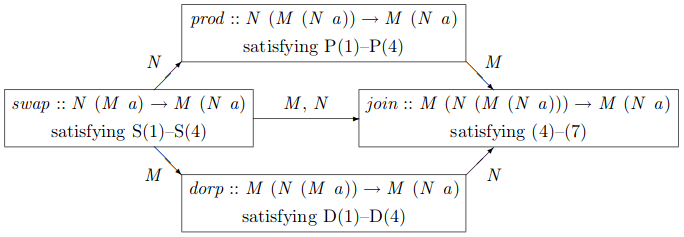
\includegraphics[width=\linewidth]{./img/graph_1}
  \label{fig:graph_1}
\end{figure}
Il secondo descrive la relazione per passare da monadi ai tre costruttori.
Questa volta gli archi descrivono proprietà richieste per ottenere il costrutto.
\begin{figure}[H]
  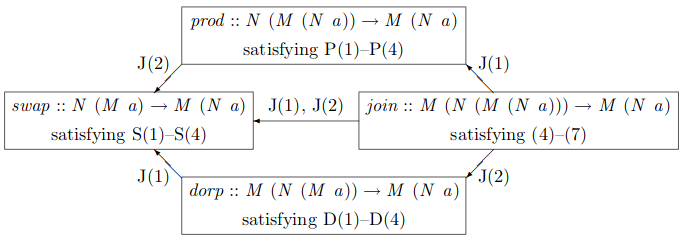
\includegraphics[width=\linewidth]{./img/graph_2}
  \label{fig:graph_2}
\end{figure}